\documentclass[10pt]{exam}
\usepackage[phy]{template-for-exam}
\usepackage{tikz}
\usepackage[top=0.2in, bottom=0.5in, left=0.5in, right=0.2in]{geometry}


\begin{document}
\pagestyle{empty}

\def\mytitle{Unit 09 Test: Sound \& Light}

\newcommand{\topmatter} {
  \hrule
  \section*{Equations}

  \begin{align*}
      v   &=  f\lambda
    & f   &= f_s \left( \frac{v\pm v_o}{v\mp v_s} \right)
    & \frac{1}{d_i} + \frac{1}{d_o} &= \frac{1}{f}
    & M &= \frac{h_i}{h_0} = \frac{-d_i}{d_o}
  \end{align*}
  %
  \vspace{-1em}
  %
  \begin{align*}
    \text{Speeds of Sound: } & 
    & \text{air: }   & \SI{340}{\meter\per\second}
    & \text{water: } & \SI{1530}{\meter\per\second}
    & \text{iron: }  & \SI{5100}{\meter\per\second}
  \end{align*}
  %
  \vspace{-2em}
  %
  \begin{align*}
    \text{Speed of Light: }
    \SI{3.0e8}{\meter\per\second}
  \end{align*}
  
  \hrule

}
\newcommand{\bottommatter}{
}

\newcommand{\drawscantron}[2]{
  \noindent
    \begin{tikzpicture}
      \node[anchor=south west] at (0,0) {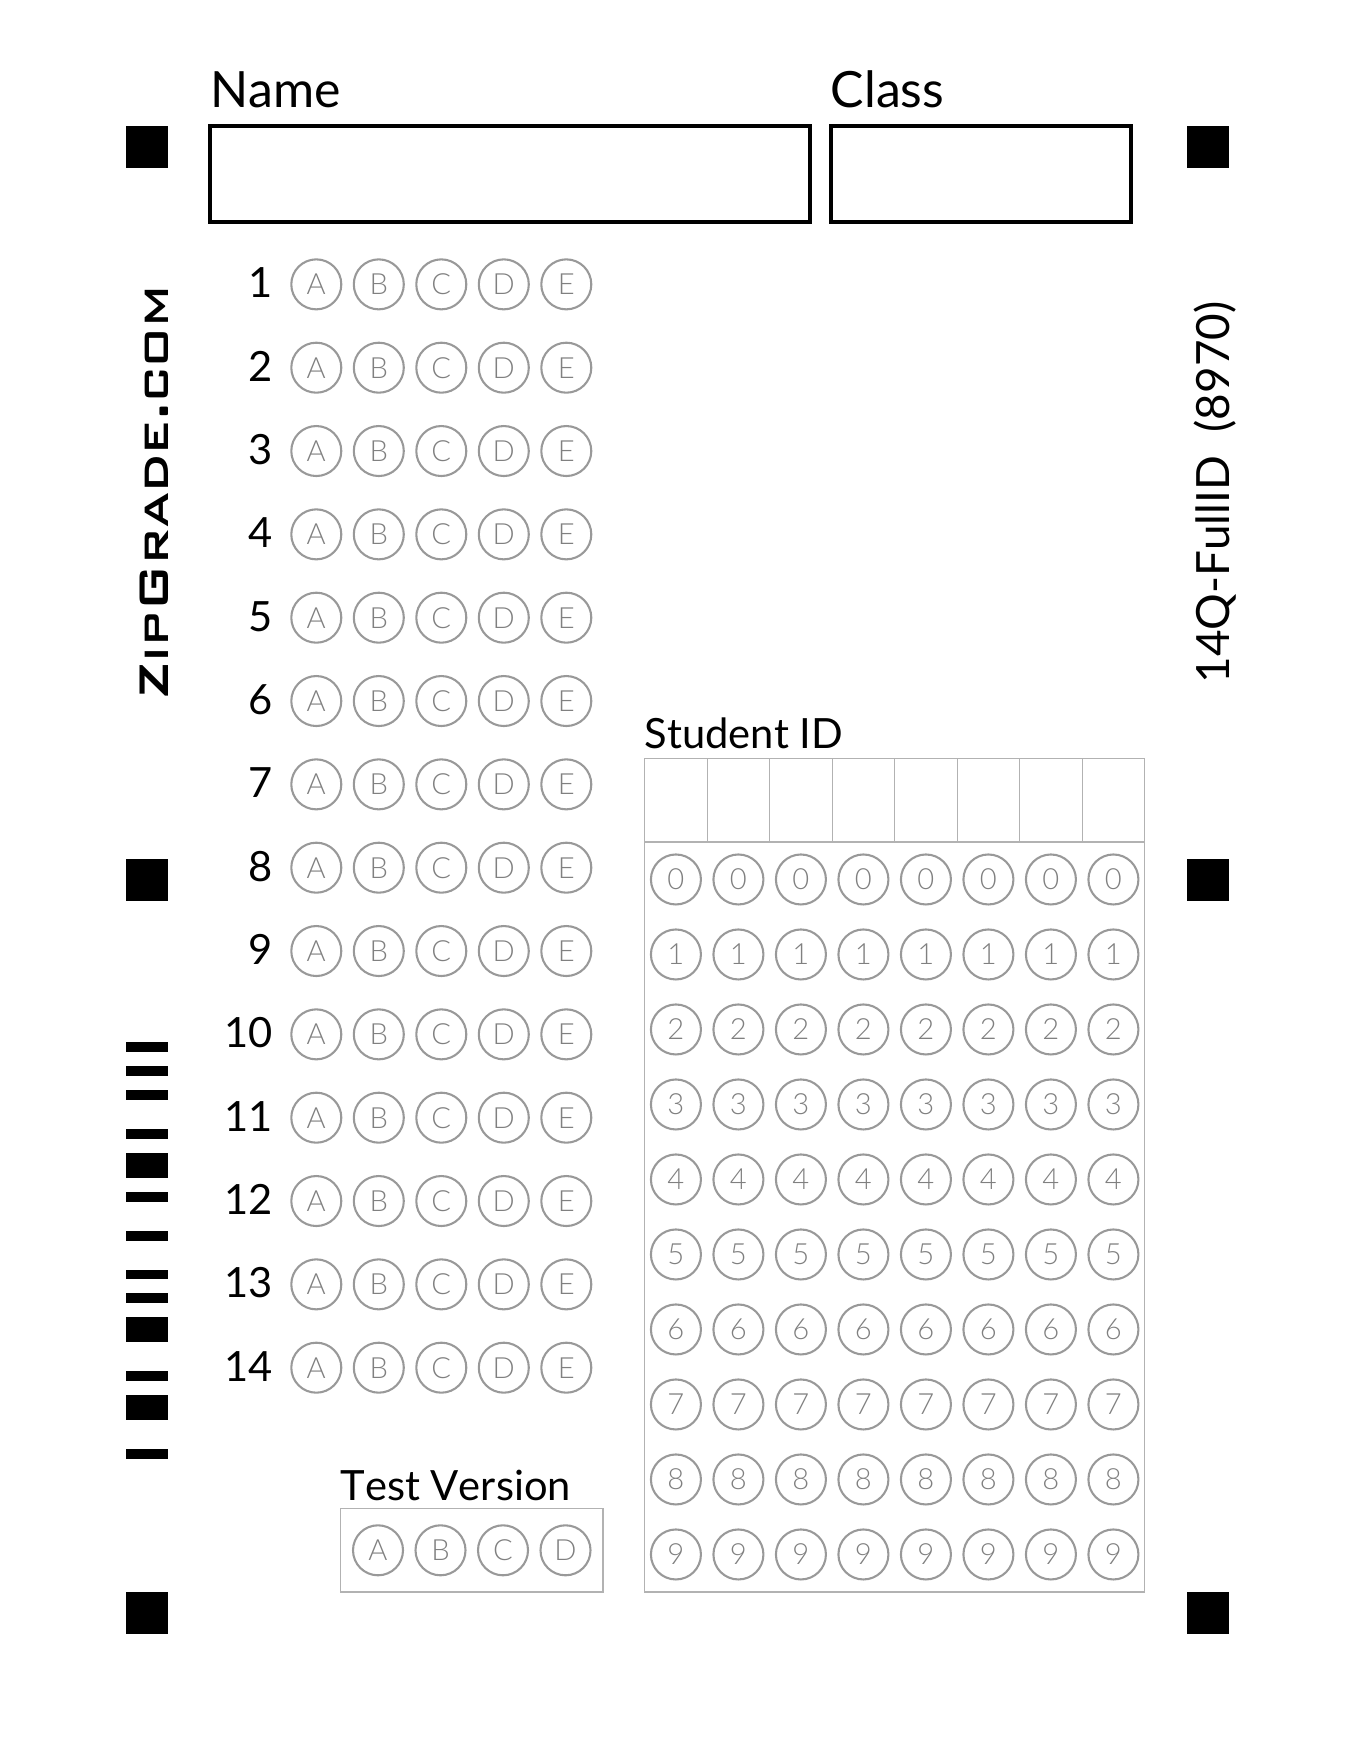
\includegraphics[width=12cm]{14Q-Full.png}};
      \fill (#1,#2) circle (0.25);
      \node[anchor=west] at (-7.5,14.5) {\Large \bf \sc \mytitle};
    \end{tikzpicture}
  
    \bottommatter
}



  \drawscantron{3.5}{2}
  \topmatter

\pagebreak

  \drawscantron{4.05}{2}
  \topmatter

\pagebreak

  \drawscantron{4.6}{2}
  \topmatter


\pagebreak

  \drawscantron{5.15}{2}
  \topmatter

\end{document}